% coaxial-jets.tex

\newpage
\section{Turbulent mixing of supersonic coaxial jets}
\label{chapter-coaxial-jets}
%
This chapter reports the validation of experiments involving the 
turbulent mixing of supersonic coaxial jets. Conducted at NASA 
Langley Research Centre, these experiments have been adopted by
the NATO Research and Technology Organisation Working Group 10 
(Subgroup 2) as a test case for their CFD development and validation
activity. More details about this test case can be found in Cutler et. al. \cite{Cutler2006}.

%------------------------------------------------------------------
\subsection{Details of flow problem}
%\label{}
%
The experimental setup used by Cutler et al. is shown 
schematically in Figure~\ref{figure-coaxial-jets-exp-setup}.
The assembly, designed to discharge two coaxial jets into 
stagnant air, was axisymmetric and consisted of an outer
body and centre body. The passage between both bodies formed
an exit nozzle for the coflow jet while the the interior passage
of the centre body formed an exit nozzle for the centre jet. Both 
%
\begin{figure}[htbp]
\begin{center}
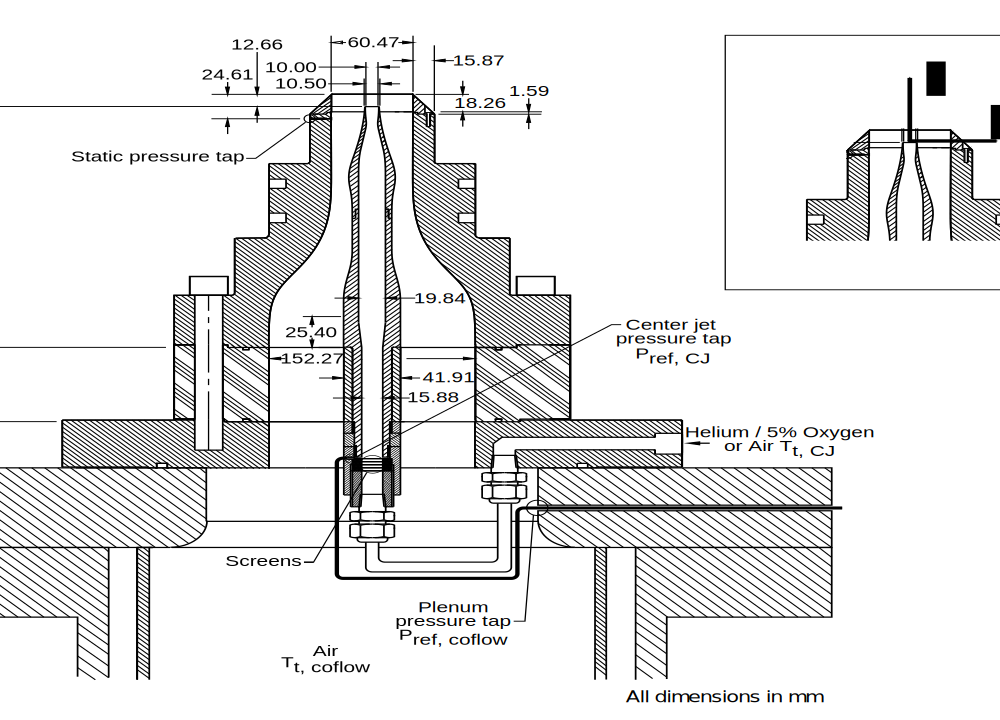
\includegraphics[width=15cm]{./chap5-coaxial-jets/figs/facility1-test.pdf}
\end{center}
\caption{Schematic diagram of experimental setup for coaxial jets test 
         case (Reprinted from \cite{Cutler2006}). Inset diagram 
         shows the coordinate system used in the Eilmer3 simulations.}
\label{figure-coaxial-jets-exp-setup}
\end{figure}
%
nozzle passages were designed using Method-of-Characteristics calculations to 
produce one-dimensional flow at the exit plane. The centre jet
consisted of a mixture of helium and oxygen (95\% He and 5\% O$_2$ by
volume, 70.4\% He and 29.6\% O$_2$ by mass), while the coflow jet 
surrounding the centre jet consisted of air. The presence of oxygen 
in the centre jet was to allow the use of an oxygen flow tagging 
technique (RELIEF) to obtain non-intrusive velocity measurements 
in the flow. Values of ambient pressure and temperature, reservoir 
pressure and temperature, and nozzle exit pressure are shown in 
Table~\ref{given-conditions-coaxial-jet}. 
%
\begin{table}[h]
  \caption{Ambient, reservoir and nozzle exit conditions}
  \label{given-conditions-coaxial-jet}
  \begin{center}
    \begin{tabular}{cccl}
      \hline\hline
      Parameter & Value   & Units \\
      \hline
      $P_{amb}$             & 101.9   & kPa \\
      $T_{amb}$             & 294.6   & K   \\
      $P_{res, \,\, coflow}$     & 580.0   & kPa \\
      $T_{res, \,\, coflow}$     & 300.0   & K   \\
      $P_{res, \,\, centrejet}$  & 614.8   & kPa \\
      $T_{res, \,\, centrejet}$  & 306.0   & K   \\
      $P_{nozzle \,\, exit, \,\, coflow}$     & 101.3   & kPa \\
      $P_{nozzle \,\, exit, \,\, centrejet}$     & 101.3   & kPa \\
      \hline \hline
    \end{tabular}
  \end{center}
\end{table}
%
Note that the exit pressure for both the coflow and centre jet
nozzles are similar. This set of experiments is considered to be 
an excellent test for the turbulence model since the streamwise 
development of the flow is dominated by turbulent stresses rather 
than pressure forces \cite{Cutler2001}.

Cylindrical pitot probes were used to measure pitot pressure. 
The mole fraction of the He-O$_2$ mixture was measured by processing 
the gas withdrawn from the flow by gas sampling probes with a hot-film 
probe-based system. The mean axial velocity and rms fluctuations were 
measured using the Raman-Excitation-plus-Laser-Induced-Electronic-Fluorescence (RELIEF) 
O$_2$ flow-tagging technique. The uncertainties in pitot pressure, 
helium-oxygen mole fractions, flow velocity, and rms fluctuations are 
$\pm$??5?\%, $\pm$1.5\%, $\pm$3\% and $\pm$3\% respectively.
Experimentally measured pitot pressure, He-O$_2$ mole fractions,
flow velocity, and turbulence intensity are compared with those
obtained from Eilmer3 simulations.

\subsection{Details of computational approach}
%\label{}
%
The grid used is shown in Figure~\ref{figure-coaxial-jets-grid}. The 
grid clustering towards the walls of both nozzles had been adjusted 
such that $y^+<1$. Grid clustering was also concentrated near the 
exit planes of both nozzles. This was done to capture the nozzle
lip shocks and expansions.
%
\begin{figure}[h]
 \centering
 \subfigure[]{
   \label{figure-coaxial-jets-overall-grid}
%   \fbox{Contents of first subfigure}
   \includegraphics[width=7cm]{./chap5-coaxial-jets/figs/grid1.pdf}
 }
 \subfigure[]{
   \label{figure-coaxial-jets-zoomed-in-grid}
%   \fbox{Contents of second subfigure}
 \includegraphics[width=7cm]{./chap5-coaxial-jets/figs/grid2.pdf}
 }
 \caption{(a) Computational mesh. (b) A close-up view of
          the mesh near exit planes of both nozzles.}
 \label{figure-coaxial-jets-grid}
\end{figure}
%
The supersonic inflow boundary condition is the preferred choice 
of inflow boundary condition for Eilmer3, rather than the subsonic 
inflow boundary condition. As such, the simulations
were started at the throats of both nozzles. Conditions at the throats
were computed by isentropically compressing the flow given in
Table~\ref{given-conditions-coaxial-jet} to sonic conditions. These inferred
conditions are shown in Table~\ref{inferred-conditions-coaxial-jet}.
%
\begin{table}[h]
  \caption{Conditions at throats of both nozzles}
  \label{inferred-conditions-coaxial-jet}
  \begin{center}
    \begin{tabular}{cccl}
      \hline\hline
      Parameter & Value   & Units \\
      \hline
      $P_{coflow,throat}$     & 306.4   & kPa \\
      $T_{coflow,throat}$     & 200.0   & K   \\
      $u_{coflow,throat}$     & 317.0   & m/s \\
      $P_{centrejet,throat}$  & 313.3   & kPa \\
      $T_{centrejet,throat}$  & 236.5   & K   \\
      $u_{centrejet,throat}$  & 759.8   & m/s \\
      \hline \hline
    \end{tabular}
  \end{center}
\end{table}
%
The turbulence intensity and turbulent-to-laminar viscosity ratio were adjusted
such that the $\sqrt{\frac{2}{3}k}$ value from the numerical simulations matched
the experimentally measured rms velocity fluctuations $\sqrt{u^{'2}}$ at the exit plane of
the nozzles (see Figure~\ref{figure-coaxial-jets-nozzle-exit-plane-d}). As described
earlier in Section~\ref{backward-facing-step-results}, a comparison between these 
values should only be treated to be approximate. The turbulence intensity used in 
this simulation was 3.5\% for the coflow jet and 2\% for the centrejet, while the 
turbulent-to-laminar viscosity ratio was 5000 for both jets. All gases used for 
this simulation were assumed to be ideal gases. In addition, a modification to 
Fick's first law of diffusion to allow for turbulent diffusion was used. The 
turbulent Prandtl number was assumed to be 0.75, as recommended in Cutler's paper.


%\subsection{Grid convergence}
%\label{}
%


\subsection{Results \& discussion}
%\label{}
%
A typical schlieren image (with vertical knife edge) from the
experiments of Cutler et. al. \cite{Cutler2006} is shown in Figure~\ref{figure-coaxial-jets-mach-contours-a},
while a contour plot of Mach number from Eilmer3 simulations is
shown in Figure~\ref{figure-coaxial-jets-mach-contours-b}.
Shock and expansion waves enamating from the 0.25-mm-thick centre
body lip (at $x$ = 0 m) into the coflowing jet can be seen in both 
experimental and numerical visualisations. Similar waves that
propagate into the centre jet in the numerical results are not 
visible in the schlieren image. It is thought that this can be
due to the low refractive index in that region \cite{Cutler2006}.
The overall qualitative agreement between the experimental
and numerical visualisations is good.  
\begin{figure}[h]
 \centering
 \subfigure[]{
   \label{figure-coaxial-jets-mach-contours-a}
%   \fbox{Contents of first subfigure}
   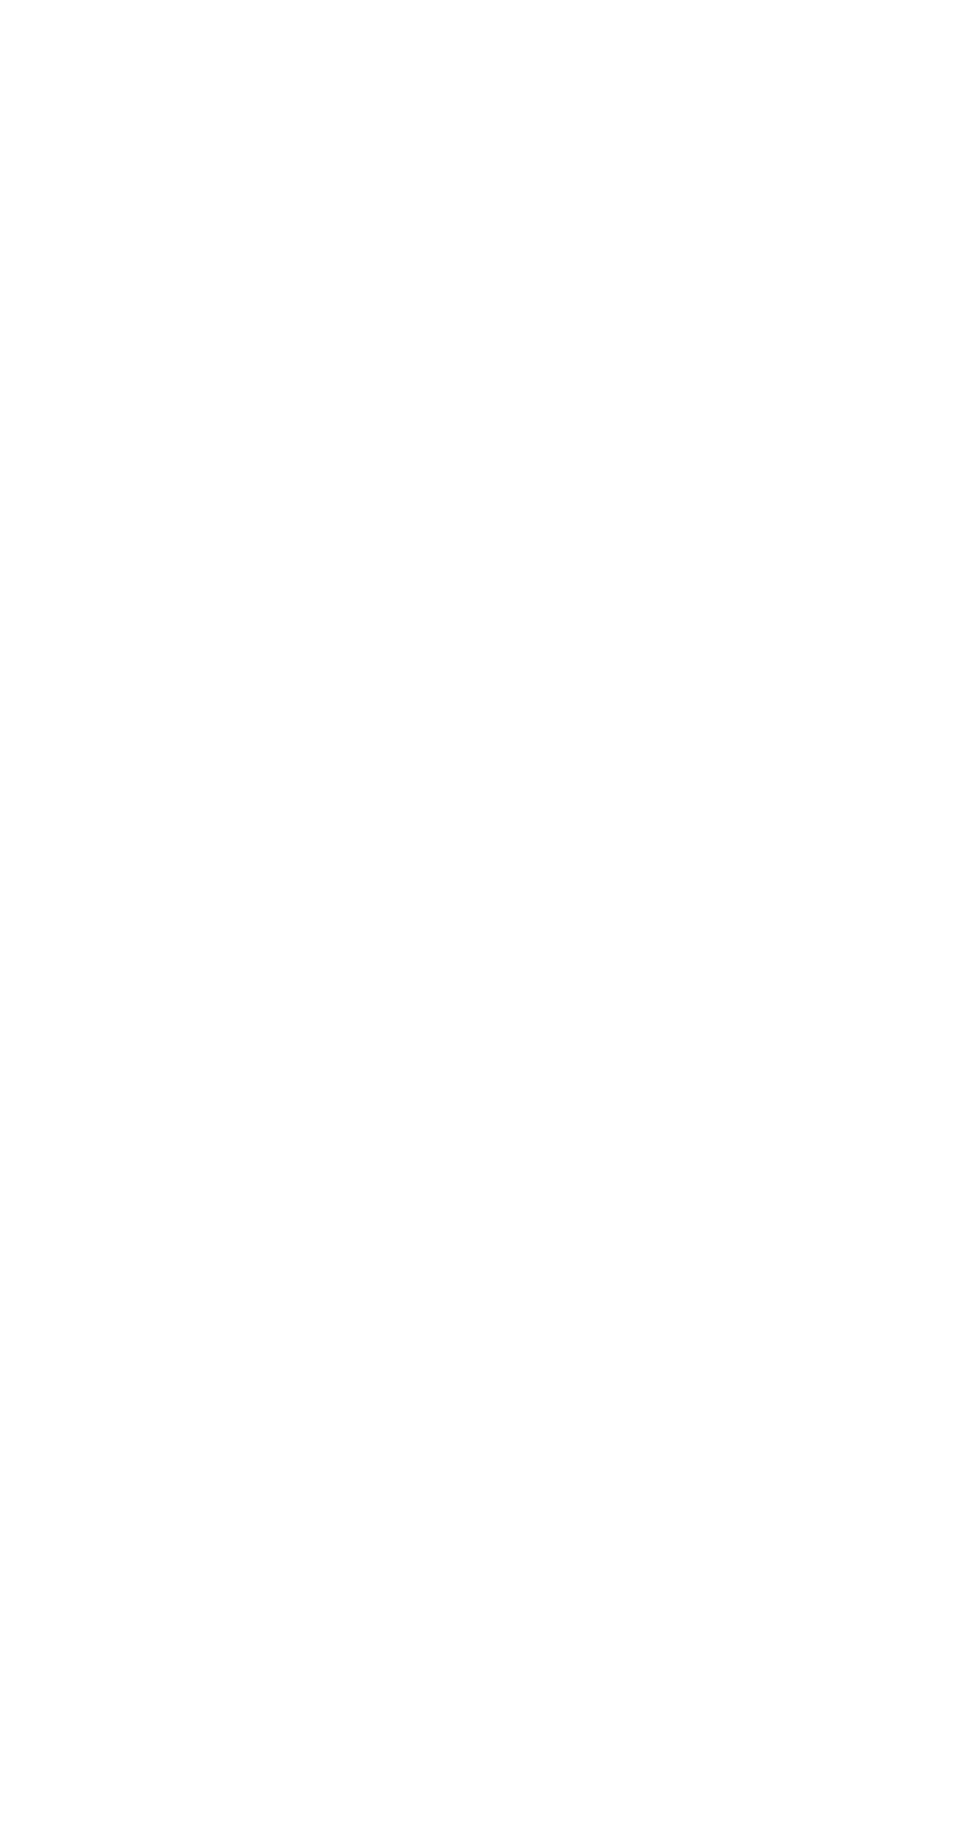
\includegraphics[width=6.5cm]{./chap5-coaxial-jets/figs/coaxial-schlieren-exp.pdf}
 }
 \subfigure[]{
   \label{figure-coaxial-jets-mach-contours-b}
%   \fbox{Contents of second subfigure}
 \includegraphics[width=6.5cm]{./chap5-coaxial-jets/figs/coaxial-schlieren-num.pdf}
 }
 \caption{Comparison between (a) experimental schlieren image and 
          (b) numerical Mach number contours}
 \label{figure-coaxial-jets-mach-contours}
\end{figure}

Figure~\ref{figure-coaxial-jets-nozzle-exit-plane} shows the comparison between
experimental data and Eilmer3 simulation results at the first 
measurement plane just downstream of the nozzles exit. The agreement
between experimental data and simulation results is excellent. This agreement 
ensures that the assumptions made for the nozzles in the simulation are valid. 
The agreement is also crucial in showing that the outflow of both jets from 
the nozzles in the experiments are accurately modelled by the Eilmer3 simulations.

Figures~\ref{figure-coaxial-jets-He-O2-mole-fractions-a} and
\ref{figure-coaxial-jets-He-O2-mole-fractions-b} show the comparison
between experimental and simulated He-O$_2$ mole fractions profiles. The 
match between the experimental and simulated He-O$_2$ mole fractions
profiles is excellent until $x$ = 0.22 m. Downstream of $x$ = 0.22 m,
the mixing appears to be overpredicted by Eilmer3, hence resulting in a lower
He-O$_2$ mole fraction near the axis of the coaxial jets. Note that at
$x$ = 0.12 m, there is a sharp discontinuity occurring in Cutler's CFD
results at $y$ = 0.008 m. This is not evident in the Eilmer3 results.
The better agreement in the Eilmer3 results with the experiments is brought
about by the use of a freestream turbulence intensity that matches that at 
the nozzle exit plane (see Figure~\ref{figure-coaxial-jets-nozzle-exit-plane-d}).

Figure~\ref{figure-coaxial-jets-pitot-pressure-a} and 
\ref{figure-coaxial-jets-pitot-pressure-b} show the comparison
between experimental and simulated pitot pressure profiles. Similar to
the comparison of He-O$_2$ mole fractions, the numerical simulations
agree with the experimental results until about $x$ = 0.22 m, where the
numerical simulations overpredict the pitot pressure near the axis of
both jets. Also, the matching of the freestream turbulence intensities
at the nozzle exit plane appear to produce a better agreement 
between the numerical simulations and experiments (compare Cutler's CFD
results and Eilmer3 results with the experimental data in Figure~\ref{figure-coaxial-jets-pitot-pressure-b-b}
at $y$ = 0.008 m). However, both numerical simulations fail to reproduce
the mixing between the coflowing jet and the ambient air (see the sharp
corners in the numerical results at $y$ = 0.023 m in Figure~\ref{figure-coaxial-jets-pitot-pressure-b-f}).

Figures~\ref{figure-coaxial-jets-u-velocity-a} and 
\ref{figure-coaxial-jets-u-velocity-b} show the comparison
between experimental and simulated  $u$-velocity profiles.
The overall agreement between the numerical and experimental $u$-velocity profiles
is reasonably good, with the exception to two discrepancies. Firstly, 
Eilmer3 does not correctly predict the $u$-velocity profiles in the mixing 
region formed by both jets (see Figure~\ref{figure-coaxial-jets-u-velocity-a}). 
Secondly, the drop in velocity below the nozzle-exit value near the axis 
of both jets is predicted to occur after $x$ = 0.153 m while it occurs 
experimentally after $x$ = 0.102 m. 

Figures~\ref{figure-coaxial-jets-rms-velocity-fluctuations-a} and
\ref{figure-coaxial-jets-rms-velocity-fluctuations-b} show the comparison
between experimentally measured rms velocity fluctuations $\sqrt{u^{'2}}$ 
and the numerically derived $\sqrt{\frac{2}{3}k}$. As mentioned earlier, the
comparison between these two quantities is valid only in truly isotropic
turbulent flows. As such, this comparison should only be treated to be
an approximate one. It can be seen in all plots that the experimentally measured
rms fluctuation levels in the coflow jet increases downstream of the exit of the 
nozzle. In contrast, Eilmer3 predicts that these levels remain constant in the 
coflow jet. Apart from this difference, the computed peak amplitudes are roughly 
consistent with the experimental data.

This validation exercise shows that Eilmer3 can be used to predict the development 
of the turbulent mixing in coaxial jets. This validation also shows that matching
the turbulence intensities to those measured experimentally at the inflow plane
aids in getting a more accurate numerical prediction of the downstream flow
development.


\begin{figure}[h]
 \centering
 \subfigure[]{
   \label{figure-coaxial-jets-nozzle-exit-plane-a}
%   \fbox{Contents of first subfigure}
   \includegraphics[width=7.5cm]{./chap5-coaxial-jets/figs/He-O2-Mole-Fractions-2D-x003.pdf}
 }
 \subfigure[]{
   \label{figure-coaxial-jets-nozzle-exit-plane-b}
%   \fbox{Contents of second subfigure}
 \includegraphics[width=7.5cm]{./chap5-coaxial-jets/figs/u-velocity-2D-x002.pdf}
 }
 \subfigure[]{
   \label{figure-coaxial-jets-nozzle-exit-plane-c}
%   \fbox{Contents of first subfigure}
   \includegraphics[width=7.5cm]{./chap5-coaxial-jets/figs/Pitot-pressure-2D-x000127.pdf}
 }
 \subfigure[]{
   \label{figure-coaxial-jets-nozzle-exit-plane-d}
%   \fbox{Contents of second subfigure}
 \includegraphics[width=7.5cm]{./chap5-coaxial-jets/figs/rms-velocity-fluctuations-2D-x002.pdf}
 }
 \caption{Comparison of flow variables at nozzle exit plane}
 \label{figure-coaxial-jets-nozzle-exit-plane}
\end{figure}

\begin{figure}[h]
 \centering
 \subfigure[]{
   \label{}
%   \fbox{Contents of first subfigure}
   \includegraphics[width=7.5cm]{./chap5-coaxial-jets/figs/He-O2-Mole-Fractions-2D-x010.pdf}
 }
 \subfigure[]{
   \label{}
%   \fbox{Contents of second subfigure}
 \includegraphics[width=7.5cm]{./chap5-coaxial-jets/figs/He-O2-Mole-Fractions-2D-x018.pdf}
 }
 \subfigure[]{
   \label{}
%   \fbox{Contents of first subfigure}
   \includegraphics[width=7.5cm]{./chap5-coaxial-jets/figs/He-O2-Mole-Fractions-2D-x028.pdf}
 }
 \subfigure[]{
   \label{}
%   \fbox{Contents of second subfigure}
 \includegraphics[width=7.5cm]{./chap5-coaxial-jets/figs/He-O2-Mole-Fractions-2D-x043.pdf}
 }
 \subfigure[]{
   \label{}
%   \fbox{Contents of first subfigure}
   \includegraphics[width=7.5cm]{./chap5-coaxial-jets/figs/He-O2-Mole-Fractions-2D-x062.pdf}
 }
 \subfigure[]{
   \label{}
%   \fbox{Contents of second subfigure}
 \includegraphics[width=7.5cm]{./chap5-coaxial-jets/figs/He-O2-Mole-Fractions-2D-x081.pdf}
 }
 \caption{He-O$_2$ mole fractions from $x$ = 0.01 m to $x$ = 0.08 m}
 \label{figure-coaxial-jets-He-O2-mole-fractions-a}
\end{figure}
%
\begin{figure}[h]
 \centering
 \subfigure[]{
   \label{}
%   \fbox{Contents of first subfigure}
   \includegraphics[width=7.5cm]{./chap5-coaxial-jets/figs/He-O2-Mole-Fractions-2D-x101.pdf}
 }
 \subfigure[]{
   \label{}
%   \fbox{Contents of second subfigure}
 \includegraphics[width=7.5cm]{./chap5-coaxial-jets/figs/He-O2-Mole-Fractions-2D-x121.pdf}
 }
 \subfigure[]{
   \label{}
%   \fbox{Contents of first subfigure}
   \includegraphics[width=7.5cm]{./chap5-coaxial-jets/figs/He-O2-Mole-Fractions-2D-x151.pdf}
 }
 \subfigure[]{
   \label{}
%   \fbox{Contents of second subfigure}
 \includegraphics[width=7.5cm]{./chap5-coaxial-jets/figs/He-O2-Mole-Fractions-2D-x181.pdf}
 }
 \subfigure[]{
   \label{}
%   \fbox{Contents of first subfigure}
   \includegraphics[width=7.5cm]{./chap5-coaxial-jets/figs/He-O2-Mole-Fractions-2D-x220.pdf}
 }
 \subfigure[]{
   \label{}
%   \fbox{Contents of second subfigure}
 \includegraphics[width=7.5cm]{./chap5-coaxial-jets/figs/He-O2-Mole-Fractions-2D-x261.pdf}
 }
 \caption{He-O$_2$ mole fractions from $x$ = 0.10 m to $x$ = 0.26 m}
 \label{figure-coaxial-jets-He-O2-mole-fractions-b}
\end{figure}

\begin{figure}[h]
 \centering
 \subfigure[]{
   \label{}
%   \fbox{Contents of first subfigure}
   \includegraphics[width=7.5cm]{./chap5-coaxial-jets/figs/Pitot-pressure-2D-x003.pdf}
 }
 \subfigure[]{
   \label{}
%   \fbox{Contents of second subfigure}
 \includegraphics[width=7.5cm]{./chap5-coaxial-jets/figs/Pitot-pressure-2D-x010.pdf}
 }
 \subfigure[]{
   \label{}
%   \fbox{Contents of first subfigure}
   \includegraphics[width=7.5cm]{./chap5-coaxial-jets/figs/Pitot-pressure-2D-x028.pdf}
 }
 \subfigure[]{
   \label{}
%   \fbox{Contents of second subfigure}
 \includegraphics[width=7.5cm]{./chap5-coaxial-jets/figs/Pitot-pressure-2D-x043.pdf}
 }
 \subfigure[]{
   \label{}
%   \fbox{Contents of first subfigure}
   \includegraphics[width=7.5cm]{./chap5-coaxial-jets/figs/Pitot-pressure-2D-x062.pdf}
 }
 \subfigure[]{
   \label{}
%   \fbox{Contents of second subfigure}
 \includegraphics[width=7.5cm]{./chap5-coaxial-jets/figs/Pitot-pressure-2D-x081.pdf}
 }
 \caption{Pitot pressure from $x$ = 0.003 m to $x$ = 0.08 m}
 \label{figure-coaxial-jets-pitot-pressure-a}
\end{figure}
%
\begin{figure}[h]
 \centering
 \subfigure[]{
   \label{}
%   \fbox{Contents of first subfigure}
   \includegraphics[width=7.5cm]{./chap5-coaxial-jets/figs/Pitot-pressure-2D-x101.pdf}
 }
 \subfigure[]{
   \label{figure-coaxial-jets-pitot-pressure-b-b}
%   \fbox{Contents of second subfigure}
 \includegraphics[width=7.5cm]{./chap5-coaxial-jets/figs/Pitot-pressure-2D-x121.pdf}
 }
 \subfigure[]{
   \label{}
%   \fbox{Contents of first subfigure}
   \includegraphics[width=7.5cm]{./chap5-coaxial-jets/figs/Pitot-pressure-2D-x151.pdf}
 }
 \subfigure[]{
   \label{}
%   \fbox{Contents of second subfigure}
 \includegraphics[width=7.5cm]{./chap5-coaxial-jets/figs/Pitot-pressure-2D-x181.pdf}
 }
 \subfigure[]{
   \label{}
%   \fbox{Contents of first subfigure}
   \includegraphics[width=7.5cm]{./chap5-coaxial-jets/figs/Pitot-pressure-2D-x220.pdf}
 }
 \subfigure[]{
   \label{figure-coaxial-jets-pitot-pressure-b-f}
%   \fbox{Contents of second subfigure}
 \includegraphics[width=7.5cm]{./chap5-coaxial-jets/figs/Pitot-pressure-2D-x261.pdf}
 }
 \caption{Pitot pressure from $x$ = 0.10 m to $x$ = 0.26 m}
 \label{figure-coaxial-jets-pitot-pressure-b}
\end{figure}

\begin{figure}[h]
 \centering
 \subfigure[]{
   \label{}
%   \fbox{Contents of first subfigure}
   \includegraphics[width=7.5cm]{./chap5-coaxial-jets/figs/u-velocity-2D-x005.pdf}
 }
 \subfigure[]{
   \label{}
%   \fbox{Contents of second subfigure}
 \includegraphics[width=7.5cm]{./chap5-coaxial-jets/figs/u-velocity-2D-x012.pdf}
 }
 \subfigure[]{
   \label{}
%   \fbox{Contents of first subfigure}
   \includegraphics[width=7.5cm]{./chap5-coaxial-jets/figs/u-velocity-2D-x027.pdf}
 }
 \subfigure[]{
   \label{}
%   \fbox{Contents of second subfigure}
 \includegraphics[width=7.5cm]{./chap5-coaxial-jets/figs/u-velocity-2D-x042.pdf}
 }
 \subfigure[]{
   \label{}
%   \fbox{Contents of first subfigure}
   \includegraphics[width=7.5cm]{./chap5-coaxial-jets/figs/u-velocity-2D-x062.pdf}
 }
 \subfigure[]{
   \label{}
%   \fbox{Contents of second subfigure}
 \includegraphics[width=7.5cm]{./chap5-coaxial-jets/figs/u-velocity-2D-x082.pdf}
 }
 \caption{$u$-velocity from $x$ = 0.005 m to $x$ = 0.08 m}
 \label{figure-coaxial-jets-u-velocity-a}
\end{figure}
%
\begin{figure}[h]
 \centering
 \subfigure[]{
   \label{}
%   \fbox{Contents of first subfigure}
   \includegraphics[width=7.5cm]{./chap5-coaxial-jets/figs/u-velocity-2D-x102.pdf}
 }
 \subfigure[]{
   \label{}
%   \fbox{Contents of second subfigure}
 \includegraphics[width=7.5cm]{./chap5-coaxial-jets/figs/u-velocity-2D-x123.pdf}
 }
 \subfigure[]{
   \label{}
%   \fbox{Contents of first subfigure}
   \includegraphics[width=7.5cm]{./chap5-coaxial-jets/figs/u-velocity-2D-x153.pdf}
 }
 \subfigure[]{
   \label{}
%   \fbox{Contents of second subfigure}
 \includegraphics[width=7.5cm]{./chap5-coaxial-jets/figs/u-velocity-2D-x190.pdf}
 }
 \subfigure[]{
   \label{}
%   \fbox{Contents of first subfigure}
   \includegraphics[width=7.5cm]{./chap5-coaxial-jets/figs/u-velocity-2D-x220.pdf}
 }
 \subfigure[]{
   \label{}
%   \fbox{Contents of second subfigure}
 \includegraphics[width=7.5cm]{./chap5-coaxial-jets/figs/u-velocity-2D-x258.pdf}
 }
 \caption{$u$-velocity from $x$ = 0.10 m to $x$ = 0.26 m}
 \label{figure-coaxial-jets-u-velocity-b}
\end{figure}

\begin{figure}[h]
 \centering
 \subfigure[]{
   \label{}
%   \fbox{Contents of first subfigure}
   \includegraphics[width=7.5cm]{./chap5-coaxial-jets/figs/rms-velocity-fluctuations-2D-x005.pdf}
 }
 \subfigure[]{
   \label{}
%   \fbox{Contents of second subfigure}
 \includegraphics[width=7.5cm]{./chap5-coaxial-jets/figs/rms-velocity-fluctuations-2D-x012.pdf}
 }
 \subfigure[]{
   \label{}
%   \fbox{Contents of first subfigure}
   \includegraphics[width=7.5cm]{./chap5-coaxial-jets/figs/rms-velocity-fluctuations-2D-x027.pdf}
 }
 \subfigure[]{
   \label{}
%   \fbox{Contents of second subfigure}
 \includegraphics[width=7.5cm]{./chap5-coaxial-jets/figs/rms-velocity-fluctuations-2D-x042.pdf}
 }
 \subfigure[]{
   \label{}
%   \fbox{Contents of first subfigure}
   \includegraphics[width=7.5cm]{./chap5-coaxial-jets/figs/rms-velocity-fluctuations-2D-x062.pdf}
 }
 \subfigure[]{
   \label{}
%   \fbox{Contents of second subfigure}
 \includegraphics[width=7.5cm]{./chap5-coaxial-jets/figs/rms-velocity-fluctuations-2D-x082.pdf}
 }
 \caption{Turbulence intensities from $x$ = 0.005 m to $x$ = 0.08 m}
 \label{figure-coaxial-jets-rms-velocity-fluctuations-a}
\end{figure}
%
\begin{figure}[h]
 \centering
 \subfigure[]{
   \label{}
%   \fbox{Contents of first subfigure}
   \includegraphics[width=7.5cm]{./chap5-coaxial-jets/figs/rms-velocity-fluctuations-2D-x102.pdf}
 }
 \subfigure[]{
   \label{}
%   \fbox{Contents of second subfigure}
 \includegraphics[width=7.5cm]{./chap5-coaxial-jets/figs/rms-velocity-fluctuations-2D-x123.pdf}
 }
 \subfigure[]{
   \label{}
%   \fbox{Contents of first subfigure}
   \includegraphics[width=7.5cm]{./chap5-coaxial-jets/figs/rms-velocity-fluctuations-2D-x153.pdf}
 }
 \subfigure[]{
   \label{}
%   \fbox{Contents of second subfigure}
 \includegraphics[width=7.5cm]{./chap5-coaxial-jets/figs/rms-velocity-fluctuations-2D-x190.pdf}
 }
 \subfigure[]{
   \label{}
%   \fbox{Contents of first subfigure}
   \includegraphics[width=7.5cm]{./chap5-coaxial-jets/figs/rms-velocity-fluctuations-2D-x220.pdf}
 }
 \subfigure[]{
   \label{}
%   \fbox{Contents of second subfigure}
 \includegraphics[width=7.5cm]{./chap5-coaxial-jets/figs/rms-velocity-fluctuations-2D-x258.pdf}
 }
 \caption{Turbulence intensities from $x$ = 0.10 m to $x$ = 0.26 m}
 \label{figure-coaxial-jets-rms-velocity-fluctuations-b}
\end{figure}
